% INTRODUCTION SECTION
\section{Introduction to ARM64 Architecture}
ARM64 (AArch64) is a 64-bit architecture developed by ARM Holdings, widely used in modern mobile devices and servers. ARM64 offers a significant register file structure, with 31 general-purpose registers and special-purpose registers such as the Program Counter (PC) and Stack Pointer (SP). These registers provide flexibility for performing low-level operations efficiently.

\subsection{Key Features}
\begin{itemize}
	\item 64-bit general-purpose registers (X0-X30).
	\item Special-purpose registers for the stack, program control, and more.
	\item Optimized function calling convention.
\end{itemize}

%	% GENERAL-PURPOSE REGISTERS SECTION
%	\section{General Purpose Registers}
%	The general-purpose registers are used to store temporary values, pass parameters to functions, and store return addresses.
%	
%	\subsection{Register Overview}
%	\begin{itemize}
	%		\item \textbf{X0-X7}: Registers used for parameter passing.
	%		\item \textbf{X8}: Indirect result register.
	%		\item \textbf{X9-X15}: Caller-saved scratch registers.
	%		\item \textbf{X19-X28}: Callee-saved registers.
	%		\item \textbf{X29 (FP)}: Frame Pointer.
	%		\item \textbf{X30 (LR)}: Link Register (return address for subroutine calls).
	%	\end{itemize}
%%	
%	\subsection{Parameter Passing Example}
%	The following example shows how function parameters are passed using ARM64 registers in C.
%	
%	\begin{tcolorbox}[title=Note]
	%		The parameters for function calls are passed in the first eight registers: X0-X7 for 64-bit values. If more than eight parameters are used, the additional ones are passed on the stack.
	%	\end{tcolorbox}
%	
%	% LINK TO C FILE WITH LISTINGS
%	Here is an example in C, which you can reference from a file named `add\_example.c`.
%	
%	\lstinputlisting[language=C, caption={Example: Function Parameter Passing}, label={lst:add_example}]{add_example.c}
%	
%	% ADDITIONAL ARM64 ASSEMBLY EXAMPLE
%	\section{ARM64 Assembly Instructions}
%	ARM64 assembly instructions operate on the general-purpose registers directly. The following is an example of adding two registers using the `add` instruction.
%	
%	\begin{lstlisting}[caption={ARM64 Assembly Example}, label={lst:assembly_example}]
	%		add x0, x0, x1   // Add contents of x0 and x1, store result in x0
	%	\end{lstlisting}
%	
%	This instruction adds the values in \texttt{x0} and \texttt{x1} and places the result in \texttt{x0}.
%	
%	% LINK TO MORE C FILES
%	You can also reference another C file demonstrating this logic in practice: `assembly\_example.c`.
%	
%	\lstinputlisting[language=C, caption={Assembly Addition in C}, label={lst:assembly_example_c}]{assembly_example.c}
%	
%	% ARM64 CALLING CONVENTIONS SECTION
%	\section{Function Calling Conventions}
%	In the ARM64 calling convention, the first eight function parameters are passed in registers X0-X7, and the return value is passed in X0. If a function requires more than eight parameters, additional values are passed on the stack.
%	
%	% CALLING CONVENTION EXAMPLE
%	The example below shows how parameters are handled in function calls:
%	
%	\lstinputlisting[language=C, caption={Calling Convention Example}, label={lst:calling_convention}]{calling_convention.c}
%	
%	% SPECIAL PURPOSE REGISTERS SECTION
%	\section{Special Purpose Registers}
%	Special-purpose registers in ARM64, like the Stack Pointer (SP) and Program Counter (PC), play a vital role in controlling the execution flow.
%	
%	\subsection{Program Counter (PC)}
%	The Program Counter (PC) holds the address of the next instruction to be executed. You can manipulate the PC to control program execution, though typically it is managed by the processor automatically.
%	
%	\subsection{Stack Pointer (SP)}
%	The Stack Pointer (SP) is used to manage the function call stack. ARM64 uses the stack to store local variables and function call return addresses.
%	
%	% FIGURES AND ILLUSTRATIONS
%	\begin{figure}[H]
	%		\centering
	%%		\includegraphics[width=0.8\textwidth]{arm64_architecture_diagram.png}
	%		\caption{Overview of ARM64 Register Structure.}
	%		\label{fig:arm64_structure}
	%	\end{figure}

% CONCLUSION SECTION
%\section{Conclusion}
%ARM64 is a powerful architecture designed for performance and efficiency. Understanding its register structure, function calling conventions, and special-purpose registers is key to writing optimized assembly and C code.

\subsection{Integer Representation in Computer Systems}

In computer systems, integers are represented using a fixed number of bits, typically grouped into bytes. This section discusses how integers are encoded, with a focus on binary representation, signed integers, and the implications of overflow.

\subsubsection{Binary Representation of Unsigned Integers}

An \emph{unsigned integer} of $n$ bits is an integer value that can take on values in the range $[0, 2^n - 1]$. In binary form, such an integer is expressed as a sum of powers of two:
\[
I = \sum_{i=0}^{n-1} b_i \cdot 2^i,
\]
where $b_i \in \{0, 1\}$ represents the $i$-th bit of the integer, with $b_0$ being the least significant bit (LSB) and $b_{n-1}$ the most significant bit (MSB).

For example, a 4-bit unsigned integer can be represented as:
\[
I = b_3 \cdot 2^3 + b_2 \cdot 2^2 + b_1 \cdot 2^1 + b_0 \cdot 2^0,
\]
which results in possible values in the range $[0, 15]$.

\begin{table}[h]
	\centering
	\begin{tabular}{|c|c|c|}
		\hline
		\textbf{Binary} & \textbf{Decimal} & \textbf{Explanation} \\ \hline
		0000            & 0                & All bits are zero           \\ \hline
		0001            & 1                & $1 \cdot 2^0$               \\ \hline
		0010            & 2                & $1 \cdot 2^1$               \\ \hline
		0111            & 7                & $1 \cdot 2^2 + 1 \cdot 2^1 + 1 \cdot 2^0$  \\ \hline
		1111            & 15               & Maximum 4-bit unsigned integer              \\ \hline
	\end{tabular}
	\caption{Example values for 4-bit unsigned integers.}
\end{table}

\subsubsection{Signed Integers: Two's Complement Representation}

In practice, computers often need to represent signed integers, i.e., integers that can be both positive and negative. One of the most widely used methods for representing signed integers is the \emph{two's complement} notation. In this system, an $n$-bit signed integer $I$ is expressed as:
\[
I = -b_{n-1} \cdot 2^{n-1} + \sum_{i=0}^{n-2} b_i \cdot 2^i.
\]
Here, $b_{n-1}$ is the sign bit, with $b_{n-1} = 0$ representing a non-negative integer, and $b_{n-1} = 1$ representing a negative integer.

\begin{table}[h]
	\centering
	\begin{tabular}{|c|c|c|}
		\hline
		\textbf{Binary (4-bit)} & \textbf{Decimal} & \textbf{Explanation}                \\ \hline
		0000                     & 0                & Zero, all bits are zero             \\ \hline
		0111                     & 7                & Largest positive number ($2^2 + 2^1 + 2^0$) \\ \hline
		1000                     & -8               & Smallest negative number ($-2^3$)   \\ \hline
		1101                     & -3               & $-2^3 + 2^2 + 2^0$                 \\ \hline
		1111                     & -1               & All bits are one ($-2^3 + 2^2 + 2^1 + 2^0$) \\ \hline
	\end{tabular}
	\caption{Example values for 4-bit signed integers using two's complement.}
\end{table}

\subsubsection{Detecting Overflow in Two's Complement Addition}

For two signed integers $x$ and $y$ represented in two's complement, overflow in addition occurs if:
\[
\begin{aligned}
	&x > 0 \quad \text{and} \quad y > 0 \quad \text{and} \quad x + y < 0, \quad \text{or} \\
	&x < 0 \quad \text{and} \quad y < 0 \quad \text{and} \quad x + y > 0.
\end{aligned}
\]
This can be efficiently detected by examining the sign bit of the result compared to the sign bits of the operands.

\begin{table}[h]
	\centering
	\begin{tabular}{|c|c|c|c|}
		\hline
		\textbf{$x$ (Binary)} & \textbf{$y$ (Binary)} & \textbf{Sum (Binary)} & \textbf{Overflow?} \\ \hline
		0110 (6)              & 0101 (5)              & 1011 (-5)             & Yes (Positive overflow) \\ \hline
		1001 (-7)             & 1110 (-2)             & 0111 (7)              & Yes (Negative overflow) \\ \hline
		0011 (3)              & 0010 (2)              & 0101 (5)              & No  \\ \hline
		1101 (-3)             & 1100 (-4)             & 1001 (-7)             & No  \\ \hline
	\end{tabular}
	\caption{Overflow detection in two's complement addition.}
\end{table}

\subsubsection{Summary}

The representation of integers on a computer is constrained by the finite number of bits available. Unsigned integers use all bits to represent non-negative values, while signed integers often employ two's complement to encode both positive and negative values. Careful handling of overflow is essential in arithmetic operations to ensure correct computational results.

\newpage

\subsection{Memory Layout in Computer Systems}

In modern computer systems, memory is divided into several distinct segments that each serve a different purpose in the execution of a program. These segments include the stack, heap, and various regions that hold code and data. This section provides a mathematical description of the layout of memory in a typical system and explains the role of each memory segment.

\subsubsection{Memory Segments}

A typical program is divided into the following memory segments:

\begin{table}[h]
	\centering
	\begin{tabular}{|c|l|}
		\hline
		\multirow{2}{*}{\textbf{Stack}} & Used for local variables, function call management, and control flow. \\
		& It grows downward in memory. \\ \hline
		\multirow{2}{*}{\textbf{Heap}} & Used for dynamic memory allocation (e.g., via \texttt{malloc}). \\ & It grows upward in memory. \\ \hline
		\textbf{.text} & Stores the program's executable instructions (machine code). \\ \hline
		\textbf{.data} & Stores initialized global and static variables. \\ \hline
		\multirow{2}{*}{\textbf{.bss}} & Stores uninitialized global and static variables. \\
		& This segment is initialized to zero at runtime. \\ \hline
		\textbf{.rodata} & Stores read-only data, such as string literals or constant variables. \\ \hline
	\end{tabular}
%	\caption{Summary of memory segments in a typical program.}
\end{table}
%\begin{itemize}
%	\item \textbf{Stack:} Used for local variables, function call management, and control flow. It grows downward in memory.
%	\item \textbf{Heap:} Used for dynamic memory allocation (e.g., via \texttt{malloc}). It grows upward in memory.
%	\item \textbf{.text:} Stores the program's executable instructions (machine code).
%	\item \textbf{.data:} Stores initialized global and static variables.
%	\item \textbf{.bss:} Stores uninitialized global and static variables. This segment is initialized to zero at runtime.
%	\item \textbf{.rodata:} Stores read-only data, such as string literals or constant variables.
%\end{itemize}

\noindent The memory layout in a typical process can be visualized as:

\begin{center}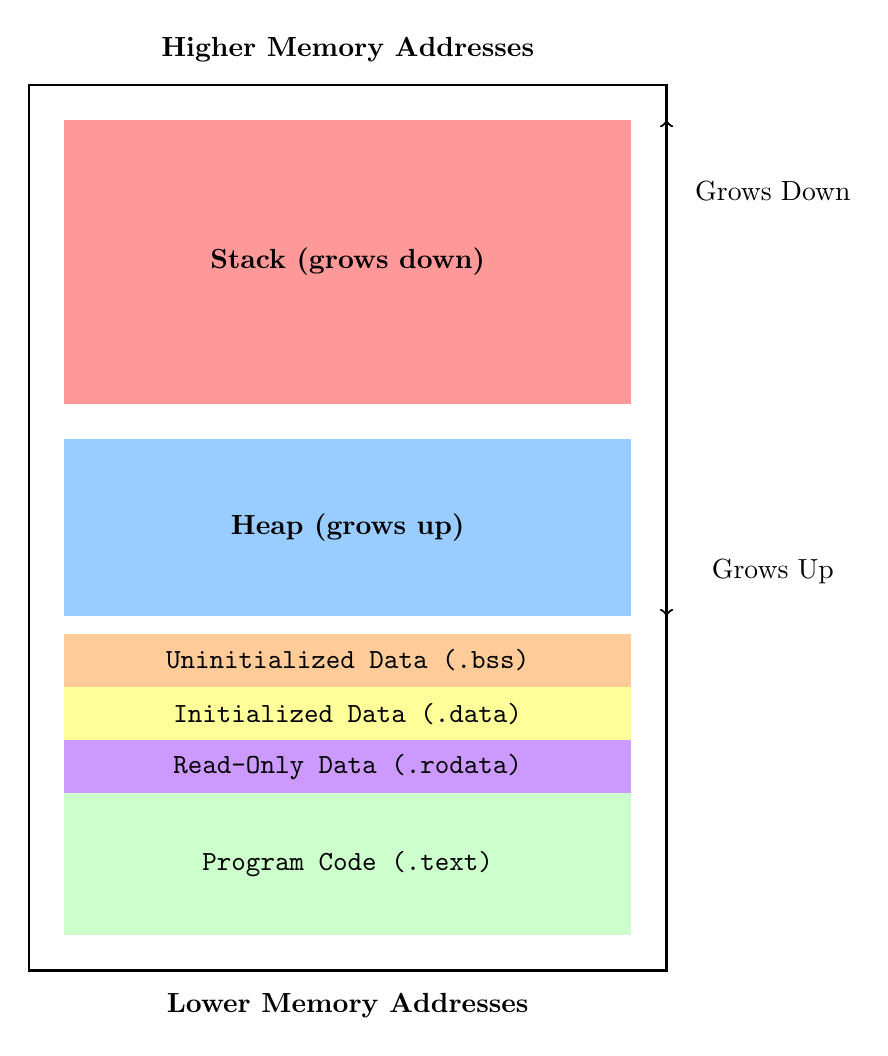
\begin{tikzpicture}[scale=.9]
	% Define colors for segments
	\definecolor{stackcolor}{RGB}{255, 153, 153}
	\definecolor{heapcolor}{RGB}{153, 204, 255}
	\definecolor{textcolor}{RGB}{204, 255, 204}
	\definecolor{datacolor}{RGB}{255, 255, 153}
	\definecolor{bsscolor}{RGB}{255, 204, 153}
	\definecolor{rodatacolor}{RGB}{204, 153, 255}
	
	% Base address
	\node at (0,10.5) {\textbf{Higher Memory Addresses}};
	\node at (0,-3.0) {\textbf{Lower Memory Addresses}};
	
	% Expanded width for rectangles (from -4 to 4)
	% Stack
	\fill[stackcolor] (-4, 5.5) rectangle (4, 9.5);
	\node at (0,7.5) {\textbf{Stack (grows down)}};
	
	% Heap
	\fill[heapcolor] (-4, 2.5) rectangle (4, 5);
	\node at (0,3.75) {\textbf{Heap (grows up)}};
	
	% BSS
	\fill[bsscolor] (-4, 1.5) rectangle (4, 2.25);
	\node at (0,1.875) {\texttt{Uninitialized Data (.bss) }};
	
	% Data
	\fill[datacolor] (-4, 0.75) rectangle (4, 1.5);
	\node at (0,1.125) {\texttt{Initialized Data (.data)}};
	
	% ROData
	\fill[rodatacolor] (-4, 0) rectangle (4, 0.75);
	\node at (0,0.375) {\texttt{Read-Only Data (.rodata)}};
	
	% Text
	\fill[textcolor] (-4, -2) rectangle (4, 0);
	\node at (0,-1) {\texttt{Program Code (.text)}};
	
	% Annotations and arrows
	\draw[thick,->] (4.5,7.5) -- (4.5,9.5);
	\node at (6,8.5) {Grows Down};
	
	\draw[thick,->] (4.5,3.75) -- (4.5,2.5);
	\node at (6,3.125) {Grows Up};
	
	% Memory boundary lines (Expand to match rectangle width)
	\draw[thick] (-4.5, -2.5) rectangle (4.5, 10);
\end{tikzpicture}\end{center}

\subsubsection{The Stack Segment}

The \emph{stack} is used to store local variables, function parameters, return addresses, and control flow information during program execution. For each function call, a \emph{stack frame} is allocated, which contains the function's local variables and bookkeeping information (such as the return address). The stack grows downward, meaning that memory addresses decrease as more data is added to the stack.

Mathematically, the size of the stack at any given time can be described as:
\[
S(t) = S_0 - \sum_{i=1}^{n} f_i,
\]
where $S_0$ is the initial stack pointer, $n$ is the number of function calls made, and $f_i$ represents the size of the $i$-th function's stack frame.

\subsubsection{The Heap Segment}

The \emph{heap} is used for dynamic memory allocation, typically requested via system calls such as \texttt{malloc} or \texttt{new}. Memory in the heap is managed manually by the programmer and persists until it is explicitly deallocated. The heap grows upward in memory.

At any point in time, the size of the heap $H(t)$ can be expressed as:
\[
H(t) = H_0 + \sum_{i=1}^{m} d_i - \sum_{j=1}^{k} r_j,
\]
where $H_0$ is the base address of the heap, $d_i$ represents the size of the $i$-th dynamically allocated block, and $r_j$ represents the size of the $j$-th deallocated block. The heap size grows with allocations and shrinks with deallocations.

\subsubsection{The .text Segment}

The \texttt{.text} segment contains the program's machine code instructions. It is typically read-only, and any attempt to write to this segment will result in an error. The size of the \texttt{.text} segment is constant after the program is loaded into memory.

Let the \texttt{.text} segment size be denoted by $T$. If the program contains $n$ instructions, each requiring $b_i$ bytes of memory, the total size of the \texttt{.text} segment is:
\[
T = \sum_{i=1}^{n} b_i.
\]

\subsubsection{The .data Segment}

The \texttt{.data} segment contains initialized global and static variables. It is writable and persistent throughout the program's execution. Each variable in this segment has an initial value, set by the program's code. The size of the \texttt{.data} segment is determined by the number and size of initialized global variables.

If a program has $n$ initialized global or static variables, and each variable $v_i$ requires $s_i$ bytes, the size of the \texttt{.data} segment is:
\[
D = \sum_{i=1}^{n} s_i.
\]

\subsubsection{The .bss Segment}

The \texttt{.bss} segment contains uninitialized global and static variables, which are automatically initialized to zero by the system at runtime. This segment does not require any space in the executable file but consumes memory at runtime.

Let the number of uninitialized variables be $n$ and let each variable $v_i$ require $s_i$ bytes. The size of the \texttt{.bss} segment is:
\[
B = \sum_{i=1}^{n} s_i.
\]

\subsubsection{The .rodata Segment}

The \texttt{.rodata} segment contains read-only data, such as constant literals and string constants. This data cannot be modified during program execution. The size of the \texttt{.rodata} segment is determined by the size of the constants stored within it.

If a program has $n$ read-only constants, and each constant $c_i$ requires $r_i$ bytes, the total size of the \texttt{.rodata} segment is:
\[
R = \sum_{i=1}^{n} r_i.
\]

\subsubsection{Memory Layout Table}

To summarize the properties of each memory segment, the following table presents a comparison of the key characteristics of each section in the memory layout:

\begin{table}[h]
	\centering
	\begin{tabular}{|c|c|c|c|}
		\hline
		\textbf{Segment} & \textbf{Purpose} & \textbf{Growth Direction} & \textbf{Writable?} \\ \hline
		\texttt{.text}   & Stores executable instructions & N/A  & No \\ \hline
		\texttt{.data}   & Stores initialized global/static variables & N/A  & Yes \\ \hline
		\texttt{.bss}    & Stores uninitialized global/static variables & N/A  & Yes \\ \hline
		\texttt{.rodata} & Stores read-only constants & N/A  & No \\ \hline
		\texttt{Heap}    & Dynamic memory allocation & Upward & Yes \\ \hline
		\texttt{Stack}   & Function call management, local variables & Downward & Yes \\ \hline
	\end{tabular}
	\caption{Summary of memory segments in a typical program.}
\end{table}

\subsubsection{Summary}

The memory layout in a computer is divided into distinct segments, each with a specific role. The stack and heap are used for dynamic and local memory management, respectively, while the \texttt{.text}, \texttt{.data}, \texttt{.bss}, and \texttt{.rodata} segments store the program's instructions, global variables, and constants. Understanding the characteristics of each segment is crucial for efficient memory management and debugging in system-level programming.

\newpage

\subsection{Performance Metrics in Computer Systems}

The performance of a computer system can be rigorously measured and analyzed using several key metrics. These metrics provide a quantitative way to evaluate the efficiency of the system in executing tasks. In this section, we will define and interrelate fundamental performance metrics such as response time, throughput, elapsed time, CPU time, instruction count, clock cycles, and discuss performance optimization via Amdahl’s Law.

\subsubsection{Response Time and Throughput}

The \emph{response time} of a system, also referred to as \emph{execution time}, is the time required to complete a single task or process. Mathematically, let $T_r$ denote the response time for a task $P$:
\[
T_r = T_{elapsed}(P),
\]
where $T_{elapsed}$ represents the total time elapsed from the start to the completion of task $P$. This includes not only the time the CPU spends on $P$, but also the time the task spends waiting for I/O or other resources.

While response time measures how long a single task takes, \emph{throughput} is concerned with the system's overall capacity to process tasks. It is defined as the number of tasks completed per unit of time. Let $X(t)$ represent the throughput over a period of time $t$, and $n$ be the number of tasks completed during this time. Then throughput is given by:
\[
X = \frac{n}{t}.
\]
Throughput and response time are inversely related in many systems, with higher throughput often implying lower response time under certain conditions.

\subsubsection{Elapsed Time and CPU Time}

The total time to execute a task, known as \emph{elapsed time}, includes both the time spent actively executing on the CPU and the time spent waiting for other resources (e.g., I/O). Let $T_{cpu}(P)$ represent the CPU time for task $P$, and $T_{io}(P)$ represent the time spent waiting for I/O. The total elapsed time $T_{elapsed}(P)$ can be written as:
\[
T_{elapsed}(P) = T_{cpu}(P) + T_{io}(P).
\]

The \emph{CPU time} is the time during which the CPU is actively executing the instructions of the program. It can be divided into two components: \emph{user CPU time}, $T_{user}$, which represents the time spent executing the program itself, and \emph{system CPU time}, $T_{system}$, which accounts for time spent executing system calls and operating system code. The total CPU time for a task $P$ is:
\[
T_{cpu}(P) = T_{user}(P) + T_{system}(P).
\]

A key factor influencing CPU time is the number of instructions executed and the efficiency of instruction processing, as discussed next.

\subsubsection{Instruction Count and Clock Cycles}

The time required for a task to complete is dependent on the number of instructions executed and the number of \emph{clock cycles} needed to execute each instruction. Let $I(P)$ represent the \emph{instruction count}—the total number of instructions executed for a task $P$. The efficiency of instruction execution is typically measured by the \emph{clock cycles per instruction} (CPI), which denotes the average number of clock cycles required to execute one instruction.

The total number of clock cycles $C_{total}$ required to execute a program $P$ is:
\[
C_{total}(P) = I(P) \cdot \text{CPI}.
\]

The CPU operates at a certain clock frequency $f$, typically measured in cycles per second (Hz). Given the total number of clock cycles $C_{total}(P)$, the CPU time $T_{cpu}(P)$ for task $P$ can be expressed as:
\[
T_{cpu}(P) = \frac{C_{total}(P)}{f} = \frac{I(P) \cdot \text{CPI}}{f}.
\]
Here, the total CPU time is directly proportional to the number of instructions, the CPI, and inversely proportional to the clock frequency.

\subsubsection{CPU Clock and Its Impact on Performance}

The \emph{CPU clock} frequency $f$ determines the rate at which the CPU executes instructions. Each clock cycle represents a discrete time step in which the CPU processes a small unit of work. Let $T_{clock}$ represent the duration of a single clock cycle, which is the reciprocal of the clock frequency:
\[
T_{clock} = \frac{1}{f}.
\]

Thus, the total time to complete a program $P$ can be expressed in terms of clock cycles and frequency, further emphasizing the critical role of the clock frequency in determining system performance.

\subsubsection{Amdahl's Law}

In practice, performance improvements often focus on optimizing certain parts of a program or task. However, the potential benefit from such optimization is limited by the fraction of the program that cannot be improved. This limitation is formalized by \emph{Amdahl's Law}, which provides an upper bound on the speedup that can be achieved by enhancing a portion of a program.

Let $p$ be the fraction of the task $P$ that can benefit from improvement, and let $k$ represent the factor by which this portion can be sped up. The overall speedup $S$ is given by:
\[
S = \frac{1}{(1 - p) + \frac{p}{k}}.
\]

In the case where $k \to \infty$ (i.e., the improved part is infinitely fast), the maximum theoretical speedup $S_{max}$ is:
\[
S_{max} = \frac{1}{1 - p}.
\]

Amdahl's Law highlights the diminishing returns of optimization when a significant fraction of the task remains unaffected by the improvement.

\subsubsection{Interrelation of Metrics}

These performance metrics—response time, throughput, CPU time, instruction count, clock cycles, and the CPU clock—are deeply interconnected. The response time of a program depends directly on its CPU time, which in turn depends on the number of instructions executed and the clock cycles per instruction. Throughput is inversely related to response time, as it reflects the system's ability to process multiple tasks in a given period.

Optimizing system performance often involves improving the CPI (through hardware efficiency), increasing the clock frequency, or reducing the number of instructions in a program. Amdahl's Law serves as a reminder that the overall system speedup is constrained by the fraction of the task that can be optimized.

\subsubsection{Summary}

The performance of a computer system can be understood through the interplay of several fundamental metrics. Response time, throughput, CPU time, and elapsed time provide different perspectives on performance. These metrics are influenced by the instruction count, clock cycles, and clock frequency, which together determine how efficiently a program is executed. Amdahl's Law further illustrates the limitations of performance improvements when only a portion of the task can be optimized. By considering these metrics in unison, we gain a comprehensive understanding of computer performance.
